\chapter{VALIDAÇÃO DOS MODELOS}
\label{validacao}
\section{\textbf{Introdução}}
Neste capítulo serão apresentadas as validações realizadas com x exemplos conhecidos amplamente na literatura.
As validações são comparações entre os resultados numéricos obtidos pela modelagem apresentada e resultados gerados por soluções analíticas conhecidas. Elas foram separadas em três grupos que representam diferentes tipos de etapas do cálculo, desse forma espera-se demonstrar a qualidade do modelo em todas as etapas e relacionar o histórico de aprendizado e desenvolvimento do código.
São utilizadas as soluções analíticas unidimensionais dos problemas para que se possa comparar os resultados pois estas são as soluções presentes na literatura. Como os resultados são obtidos para problemas bidimensionais é preciso fazer a comparação entre resultados tomando uma seção da solução como referência, usualmente perto do meio. Essa adaptação dos dados gera uma aproximação dos resultados.

O primeiro grupo são os problemas em sólidos, que buscam confirmar a construção correta das matrizes de elementos, a aplicação apropriada dos diferentes tipos de condições de contorno e a solução de um modelo mais simples.
O segundo grupo trata dos exemplos de problemas com fluidos. 
Nesta etapa verifica-se novamente a construção das matrizes e aplicação das condições de contorno, 
porém o foco principal destes exemplos é validar o modelo e analisar as restrições de aplicabilidade.
Para o terceiro e último grupo de validações são trabalhados problemas clássicos em partículas.
São realidados testes para validar cada força trabalhando isoladamente, dessa forma facilita-se a correção pontual no modelo e pode-se comprovar com maior certeza a influência correta das forças.

Calculam-se os erros entre os resultados em cada ponto para se verificar a acurácia do modelo e sua implementação.
O erro relativo entre a solução numérica e analítica é calculado pela equação:
\begin{equation}
    er_i = \frac{(val_a)_i - (val_n)_i}{(val_a)_i}
    \label{error_eq} 
\end{equation}
Onde $(val_a)_i$ é o valor encontrado pela solução analítica e $(val_n)_i$ é o valor encontrado pela solução numérica, ambos encontrados no ponto $i$.

São calculados também a média dos erros relativos:
\begin{equation}
    er_{mean} = \frac{1}{N}\sum_{i=0}^{N} er_i
    \label{error_mean}
\end{equation}

E o desvio padrão dos erros relativos:
\begin{equation}
    er_{std} = \sqrt{\frac{1}{N}\sum_{i=0}^{N} (er_i-er_{mean})^2}
    \label{error_std} 
\end{equation}

A execução do código e computação dos resultados foram realizados em um computador de uso pessoal com as seguintes especificações:
\begin{itemize}
    \item Dell Latitude E6410 com processador Intel® Core™ i5 CPU M 520 2.40GHz com 4 núcloes e 4Gb de memória RAM.
          O sistema operacional ubuntu 16.04 LTS e compilador Python 3.5.
\end{itemize}

%---------------------------------------------------------------------------------------------------------Validação de sólidos
\section{\textbf{Validações de Problemas em Sólidos}}
%---------------------------------------------------------------------------------------------Primeiro Exemplo
\subsection{\textbf{Equação de Laplace com Condições de Contorno de Dirichlet}}
\label{sec_laplace_dir}
O problema de troca de calor em uma placa é um dos exemplos clássicos utilizados para estudar as equações de transmissão de calor em sólidos. O mais simples destes é uma barra unidimensional sem geração de calor onde a temperatura é conhecida nas extremidades.
Como a malha do código foi desenvolvida para solução de problemas bidimensionais, cria-se um problema bidimensional com condições de contorno equivalentes e extrai-se uma seção para que se possa comparar os resultados.

A equação de governo desta situação é a equação de Laplace \ref{laplace_d_perm_eq} para sólidos em estado permanente.
\begin{equation}
    \nabla^2 T = 0
    \label{laplace_d_perm_eq} 
\end{equation}
Onde T é a temperatura na placa.

E a solução analítica do problema unidimensional associado é \ref{laplace_d_sol}.
\begin{equation}
    T(x) = \dfrac{T_L-T_0}{L} x + T_0
    \label{laplace_d_sol}
\end{equation}
Onde $L$ é o comprimento da barra, $T_0$ e $T_L$ são, respectivamente, os valores da temperatura em $x=0$ e $x=L$.

Os parâmetros do problema unidimensional são definidos como:
\begin{itemize}
    \item $x\in [0,1]m$
    \item $T(0) = 0^{\circ}C$
    \item $T(1) = 1^{\circ}C$
\end{itemize}

As condições do problema bidimensional equivalente, ver \ref{laplace_d_bc}, onde a seção tomada será em $x=0.5m$, é dado por:
\begin{itemize}
    \item $x,y\in [0,1]m$
    \item $T(0,y) = 0^{\circ}C$
    \item $T(1,y) = 1^{\circ}C$
    \item $\dfrac{\partial T}{\partial n}(x,0) = 0^{\circ}C/m$
    \item $\dfrac{\partial T}{\partial n}(x,1) = 0^{\circ}C/m$
\end{itemize}

\begin{figure}[H]
    \centering
    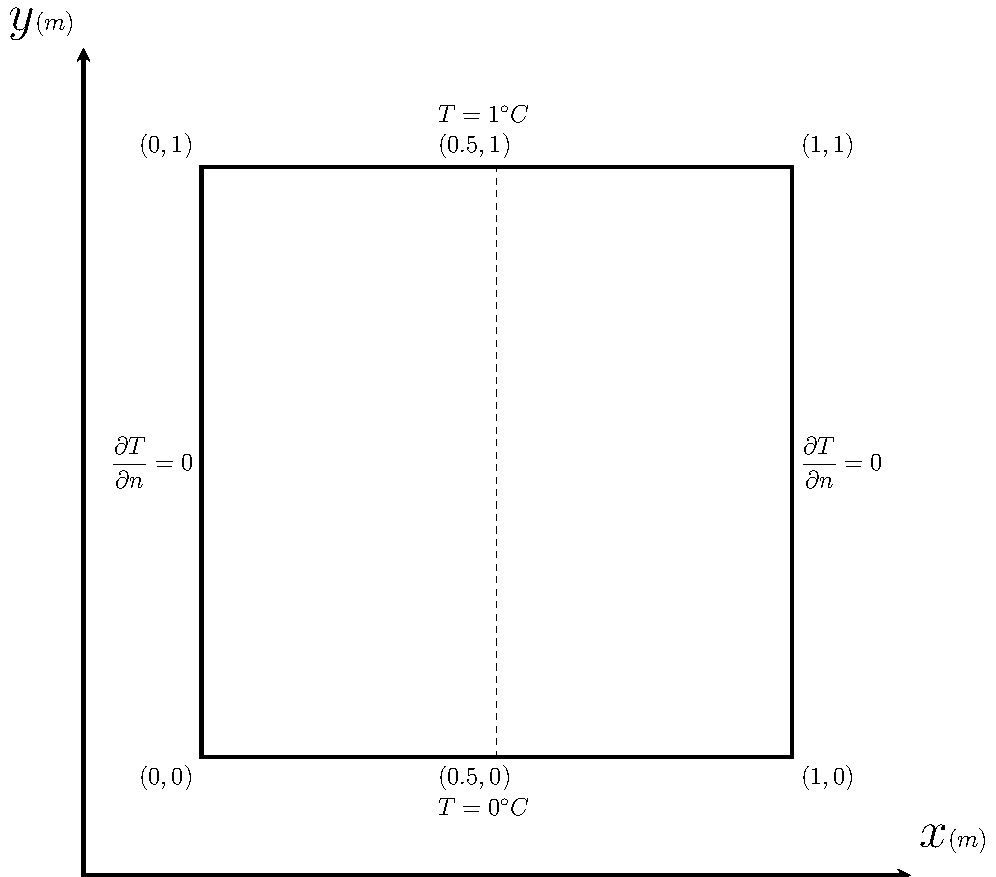
\includegraphics[width=.7\linewidth]{figures/laplace_dirichlet_boundary_conditions.pdf}
    \caption{Condições de contorno da placa para o problema de Laplace \ref{sec_laplace_dir}.}
    \label{laplace_d_bc}
\end{figure}

Para os cálculos deste exemplo foi utilizada uma malha com 768 elementos e 417 nós.
\begin{figure}[H]
    \centering
    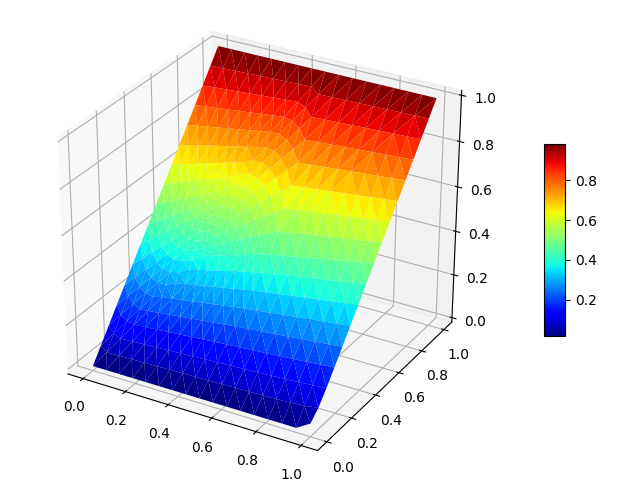
\includegraphics[width=.5\linewidth]{figures/laplace_dirichlet_permanent_3d.png}
    \caption{Distribuição de temperaturas na placa da solução permanente da equação de Laplace \ref{sec_laplace_dir}.}
    \label{laplace_d_3d}
\end{figure}

A comparação entre os resultados da solução analítica \ref{laplace_d_sol} e a solução numérica \ref{laplace_d_3d}:
\begin{figure}[H]
    \centering
    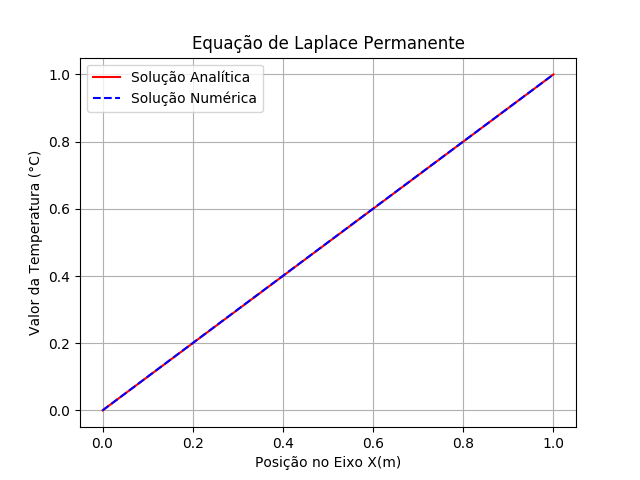
\includegraphics[width=.7\linewidth]{figures/laplace_dirichlet_permanent_comparison.png}
    \caption{Comparação de resultado das soluções númerica e analítica do caso permanente da equação de Laplace \ref{sec_laplace_dir}.}
    \label{laplace_d_perm_comp}
\end{figure}
Onde o erro relativo médio encontrado foi de $0.1136\%$ e com desvio padrão de $0.0008\%$.

Ao solucionar o mesmo problema introduzindo um termo temporal a equação de governo, pode-se verificar a evolução de comportamento da temperatura ao longo do tempo.
\begin{equation}
    \dfrac{\partial T}{\partial t} + k\nabla^2 T = 0
    \label{laplace_d_trans_eq} 
\end{equation}
Onde $k$ é o coeficiente de condutividade térmica da placa.

Porém ao longo dos passos de tempo, a solução se aproxima de um problema permanente, portanto pode-se fazer a comparação dos resultados obtidos neste exemplo com os valores da solução analítica \ref{laplace_d_sol}, tomando-se que $t\rightarrow \infty$.

Foi utilizado um critério de parada de $10^{-5}$ de variação de valores entre intervalos de tempo para obtenção dos resultados em \ref{laplace_d_trans_comp}.
As condições iniciais $t=0s$ atribuídas aos pontos sem condição de contorno foram de um valor inicial de $0^{\circ}C$.
\begin{figure}[H]
    \centering
    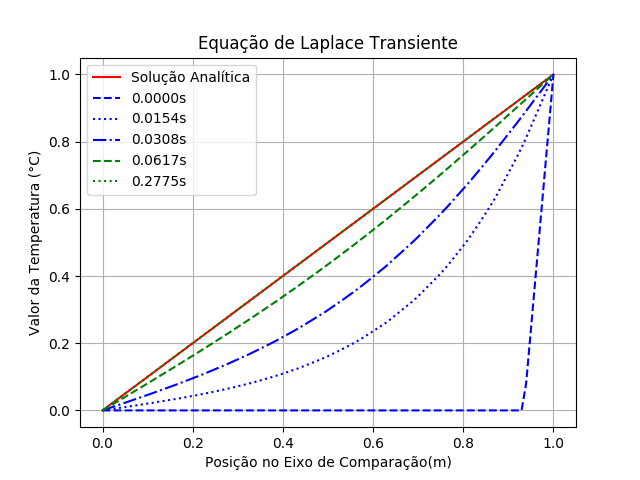
\includegraphics[width=.7\linewidth]{figures/laplace_dirichlet_transient_comparison.png}
    \caption{Comparação de resultado das soluções númerica e analítica ao longo do tempo do caso transiente da equação de Laplace \ref{sec_laplace_dir}.}
    \label{laplace_d_trans_comp}
\end{figure}
Onde o erro relativo médio encontrado foi de $0.1092\%$ e com desvio padrão de $0.0008\%$.


%---------------------------------------------------------------------------------------------Segundo Exemplo
\subsection{\textbf{Equação de Poisson com Condições de Contorno de Dirichlet}}
\label{sec_poisson_dir}
Neste problema busca-se estudar o comportamento de uma placa com geração de calor em seu domínio e temperaturas fixas nas laterais.
Novamente, para permitir a comparação de resultados, é extraída uma seção da placa para observar os resultados como um problema unidimensional.

A equação deste caso é denomidada equação de Poisson \ref{poisson_d_perm_eq}, tomada para um problema permanente, ou seja sem variação no tempo.
\begin{equation}
    -k\nabla^2 T = Q
    \label{poisson_d_perm_eq} 
\end{equation}
Onde $Q$ é a geração de calor na placa.

A solução analítica para o caso de uma barra unidimensional é descrita em \ref{poisson_d_sol}
\begin{equation}
    T(x) = \dfrac{Q}{2k}\Big(-x^2 + L x\Big) + \dfrac{T_L-T_0}{L} x + T_0
    \label{poisson_d_sol} 
\end{equation}

As condições do problema bidimensional, ver \ref{poisson_d_bc}, onde a seção de comparação será em $x=0.5m$, são dadas por:
\begin{itemize}
    \item $x,y\in [0,1]m$
    \item $T(0,y) = 0^{\circ}C$
    \item $T(1,y) = 0^{\circ}C$
    \item $\dfrac{\partial T}{\partial n}(x,0) = 0^{\circ}C/m$
    \item $\dfrac{\partial T}{\partial n}(x,1) = 0^{\circ}C/m$
    \item $Q(x,y) = 40W/m^2$
    \item $k = 5W/K$
\end{itemize}

\begin{figure}[H]
    \centering
    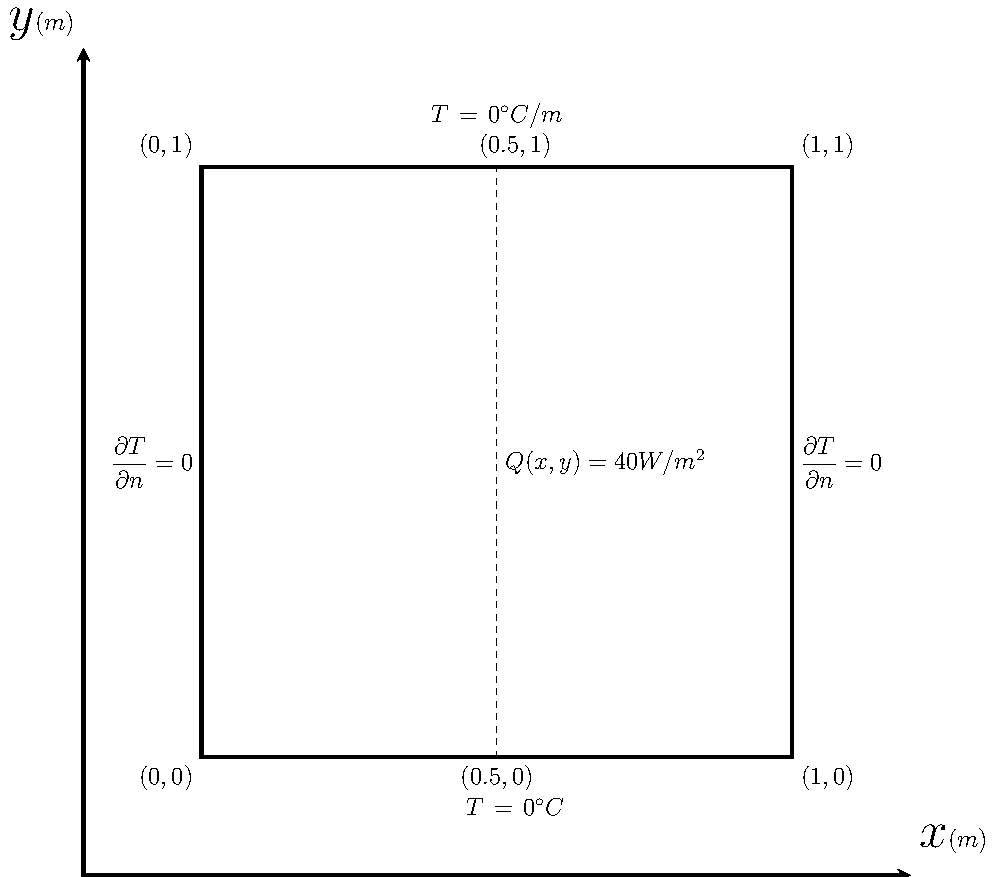
\includegraphics[width=.7\linewidth]{figures/poisson_dirichlet_boundary_conditions.pdf}
    \caption{Condições de contorno da placa para o problema de Poisson \ref{sec_poisson_dir}.}
    \label{poisson_d_bc}
\end{figure}

Novamente foi utilizada uma malha com 768 elementos e 417 nós.
\begin{figure}[H]
    \centering
    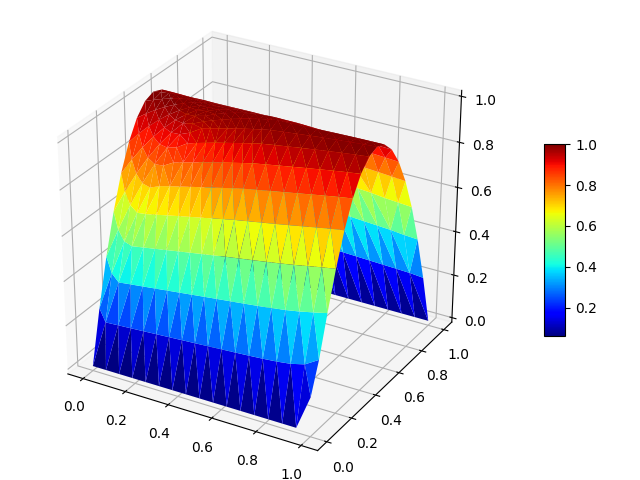
\includegraphics[width=.5\linewidth]{figures/poisson_dirichlet_permanent_3d.png}
    \caption{Distribuição de temperaturas na placa da solução do problema permanente de Poisson \ref{sec_poisson_dir}.}
    \label{poisson_d_3d}
\end{figure}

A comparação entre os resultados da solução analítica \ref{poisson_d_sol} e a solução numérica \ref{poisson_d_3d}:
\begin{figure}[H]
    \centering
    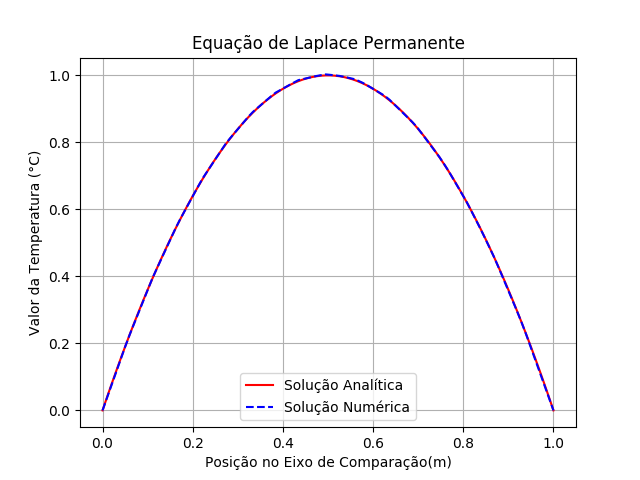
\includegraphics[width=.7\linewidth]{figures/poisson_dirichlet_permanent_comparison.png}
    \caption{Comparação de resultado das soluções númerica e analítica do problema permanete de Poisson \ref{sec_poisson_dir}.}
    \label{poisson_d_perm_comp}
\end{figure}
Onde o erro relativo médio encontrado foi de $-0.323\%$ e com desvio padrão de $0.0101\%$.

E o resultado com o termo de tempo $\dfrac{\partial T}{\partial t}$ tendendo a um estado permanente, novamente foi utilizado um critério de parada de $10^{-5}$ de diferença nos valores entre os intervalos de tempo nos resultados em \ref{poisson_d_trans_comp}.
As condições iniciais $t=0s$ atribuídas aos pontos sem condição de contorno foram de um valor inicial de $0^{\circ}C$.

\begin{figure}[H]
    \centering
    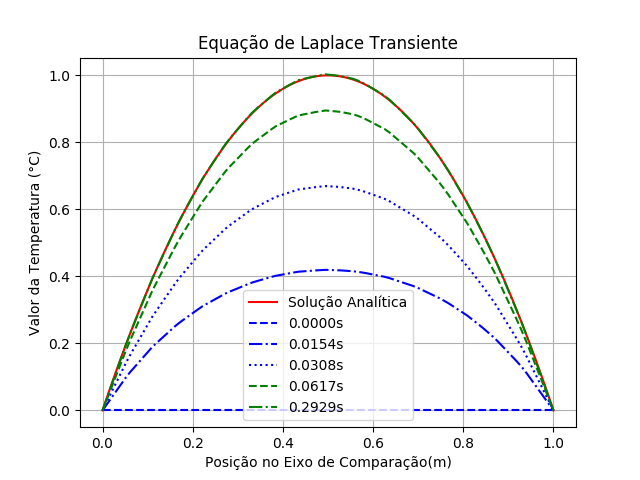
\includegraphics[width=.7\linewidth]{figures/poisson_dirichlet_transient_comparison.png}
    \caption{Comparação de resultado das soluções númerica e analítica do problema transiente de Poisson \ref{sec_poisson_dir}.}
    \label{poisson_d_trans_comp}
\end{figure}
Onde o erro relativo médio encontrado foi de $-0.325\%$ e com desvio padrão de $0.0101\%$.

%---------------------------------------------------------------------------------------------Terceiro Exemplo
\subsection{\textbf{Equação de Poisson com Condições de Contorno de Dirichlet e Neumann}}
\label{sec_poisson_neu}
Este caso foi escolhido para validar a solução de problemas com condições de contorno de Neumann.
Trata-se de uma placa com temperatura fixa em uma das paredes e no lado oposto é defido um valor para a taxa de troca de calor presente.
Toma-se uma seção da placa para observar os resultados e compará-los com um problema unidimensional de uma barra com as mesmas condições presentes.

A equação de troca térmica é novamente a equação de Poisson \ref{poisson_d_perm_eq}, com solução analítica para uma barra unidimensional \ref{poisson_n_sol}.
\begin{equation}
    T(x) = \dfrac{Q}{k}\Big(\dfrac{-x^2}{2} + L x\Big) + dT_L x + T_0
    \label{poisson_n_sol} 
\end{equation}
Onde $dT_L$ é o valor da taxa de troca térmica na extremidade $x=L$.

As condições do problema bidimensional, ver \ref{poisson_n_bc}, onde a seção tomada será em $x=0.5m$, são dadas por:
\begin{itemize}
    \item $x,y\in [0,1]m$
    \item $T(0,y) = 0^{\circ}C$
    \item $\dfrac{\partial T}{\partial n}(1,y) = 1^{\circ}C/m$
    \item $\dfrac{\partial T}{\partial n}(x,0) = 0^{\circ}C/m$
    \item $\dfrac{\partial T}{\partial n}(x,1) = 0^{\circ}C/m$
    \item $Q(x,y) = -7W/m^2$
    \item $k = 5W/K$
\end{itemize}

\begin{figure}[H]
    \centering
    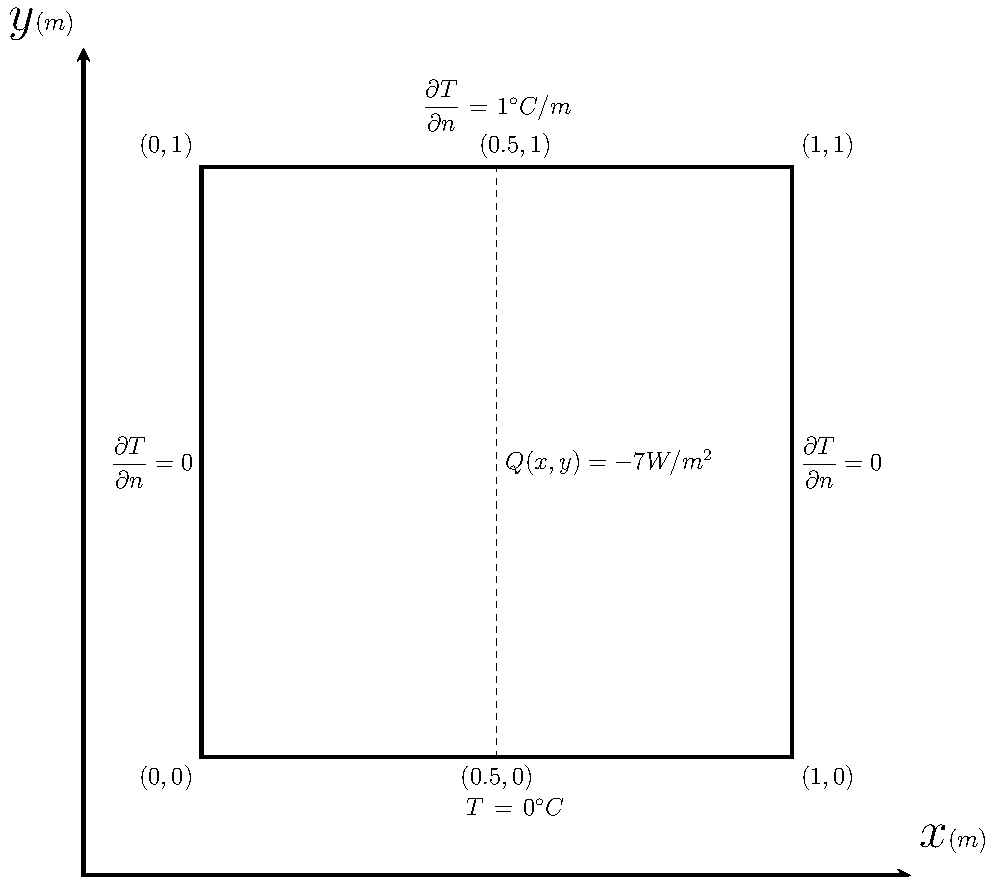
\includegraphics[width=.7\linewidth]{figures/poisson_neumann_boundary_conditions.pdf}
    \caption{Condições de contorno da placa para o problema de Poisson \ref{sec_poisson_neu}.}
    \label{poisson_n_bc}
\end{figure}

Mais uma vez foi utilizada uma malha com 768 elementos e 417 nós.
\begin{figure}[H]
    \centering
    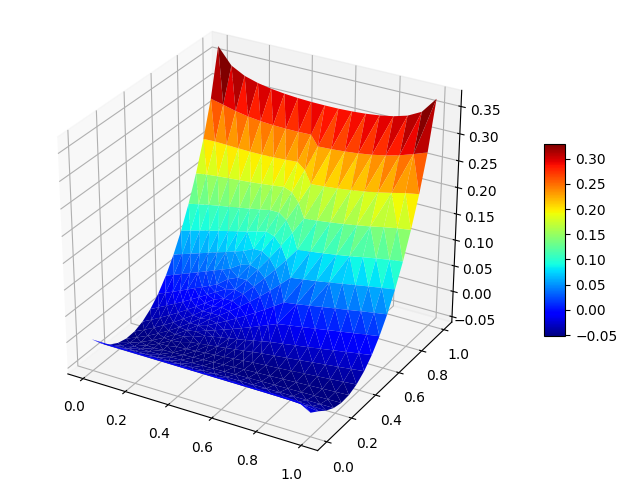
\includegraphics[width=.5\linewidth]{figures/poisson_neumann_permanent_3d.png}
    \caption{Distribuição de temperaturas na placa da solução do problema permanente de Poisson \ref{sec_poisson_neu}.}
    \label{poisson_n_3d}
\end{figure}

A comparação entre os resultados da solução analítica \ref{poisson_n_sol} e a solução numérica \ref{poisson_n_3d}:
\begin{figure}[H]
    \centering
    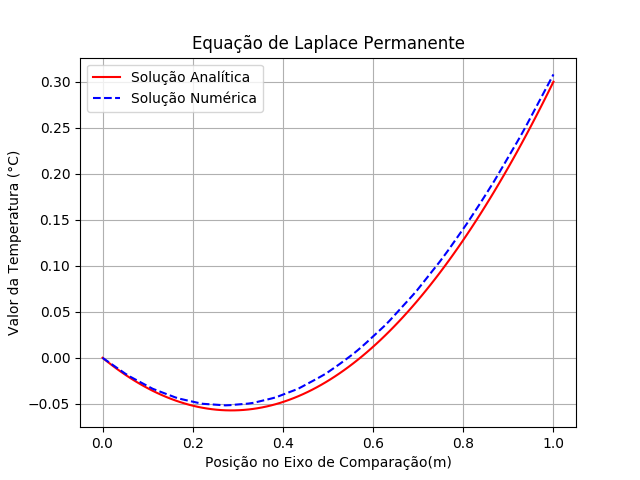
\includegraphics[width=.7\linewidth]{figures/poisson_neumann_permanent_comparison.png}
    \caption{Comparação de resultado das soluções númerica e analítica do problema permanete de Poisson \ref{sec_poisson_neu}.}
    \label{poisson_n_perm_comp}
\end{figure}
Onde o erro relativo médio encontrado foi de $-0.427\%$ e com desvio padrão de $0.8414\%$.

Para o resultado transiente foi utilizado um critério de parada de $10^{-5}$.
As condições iniciais $t=0s$ atribuídas aos pontos sem condição de contorno foram de um valor inicial de $0^{\circ}C$.

\begin{figure}[H]
    \centering
    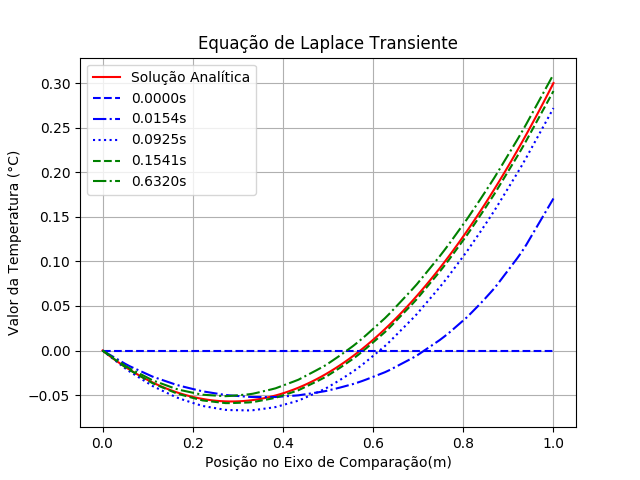
\includegraphics[width=.7\linewidth]{figures/poisson_neumann_transient_comparison.png}
    \caption{Comparação de resultado das soluções númerica e analítica do problema transiente de Poisson \ref{sec_poisson_neu}.}
    \label{poisson_n_trans_comp}
\end{figure}
Onde o erro relativo médio encontrado foi de $-0.31\%$ e com desvio padrão de $0.9205\%$.

%---------------------------------------------------------------------------------------------------------Validação de fluidos
\section{\textbf{Validações de Problemas em Fluídos}}
%---------------------------------------------------------------------------------------------Primeiro Exemplo
\subsection{\textbf{Escoamento de Hagen-Poiseuille}}
%---------------------------------------------------------------------------------------------Segundo Exemplo
\subsection{\textbf{Escoamento de Couette}}
%---------------------------------------------------------------------------------------------Terceiro Exemplo
\subsection{\textbf{Escoamento de Cavidade (\it{Lid-Driven Cavity Flow})}}


%---------------------------------------------------------------------------------------------------------Validação de partículas
\section{\textbf{Validações de Problemas em Partículas}}
%---------------------------------------------------------------------------------------------Primeiro Exemplo
\subsection{\textbf{Força Gravitacional}}
%---------------------------------------------------------------------------------------------Segundo Exemplo
\subsection{\textbf{Força de Arrasto}}
%---------------------------------------------------------------------------------------------Terceiro Exemplo
\subsection{\textbf{Força de Sustentação}}